\documentclass[10pt]{report}
\usepackage{fullpage}
\usepackage{amsmath}
\usepackage{amsfonts}
\usepackage{amssymb}
\usepackage[version=4]{mhchem}
\usepackage{stmaryrd}
\usepackage{graphicx}
\usepackage{array}
\usepackage{babel}
\usepackage{caption}
\usepackage{color}
\usepackage{float}
\usepackage{parskip}
\usepackage{physics}
\usepackage{subcaption}
\usepackage{caption}
\captionsetup{justification=centering}
\usepackage[export]{adjustbox}

\graphicspath{ {./images/} }

\title{Two-Antenna GPS/INS }
\author{Popescu Ervin-Adrian\\444C}
\date{}


\begin{document}
\maketitle
\section*{Introducere}
Pentru a aborda problemele privind erorile de model dinamic și, în special, măsurarea
valorilor outlier, propunem o abordare adaptativă robustă pentru integrarea GPS/INS LC cu două antene în care metoda IAE este utilizată pentru a proiecta un factor pentru covarianța adaptivă. Mai multe ecuații în cauză cu IAE dezavantajele sunt derivate pentru a explica și depăși problemele numerice și de feedback ale
integrarea GPS/INS cu două antene cauzată de valori outlier de măsurare și incertitudini de stare necunoscute,
și o reconfigurare adaptivă pentru covarianța zgomotului de măsurare în funcție de fiabilitatea măsurării  este proiectată. Proprietățile de dorit ale abordării propuse sunt rezumate după cum urmează:
\begin{itemize}
  \item Modificarea adaptivă a covarianței zgomotului poate trata erorile de model dinamic și măsurarea
        perturbare pentru a reduce impactul lor asupra estimării de stare, mai ales atunci când statisticile măsurătorilor și zgomotului prognozat trebuie adaptate. Cu actualizarea filtrului, feedbackul pozitiv și problemele numerice pot fi reduse prin cuantificarea zgomotului de măsurare statistică la un nivel mai granular pe baza cuantificării corespunzătoare ale fiabilității măsurătorii în cazul valorilor outlier ale măsurătorilor.
  \item Metoda propusă poate cuantifica cu precizie fiabilitatea măsurătorilor. Este o metodă de reglementare bazată pe dovezi, cu avantajul atenuării impactului perturbării inovației. În plus față de
        stabilitatea asigurată a actualizării filtrului, performanța ecuației de măsurare augmentată în feedback-ul de eroare de stare pentru măsurători prețioase este îmbunătățită.
\end{itemize}

Lucrarea este organizată după cum urmează. O prezentare generală a algoritmului integrat GPS/INS cu două antene este oferită în Secțiunea 2. În Secțiunea 3, este discutată modificarea adaptivă a covarianței zgomotului. Experimentul de teren și rezultatele pentru diferite scheme sunt comparate în Secțiunea 4 pentru a verifica superioritatea abordării propuse în comparație cu metodele existente. În final, sunt trase câteva concluzii ale acestei lucrări.

\subsection*{Inertial Dynamic Model}
Modelul dinamic inerțial este derivat din modelul de eroare Psi-Angle bazat pe ecuații diferențiale de eroare INS și rezumat ca:

\begin{equation}
  \begin{aligned}
    \delta \dot{r} & =-\omega_{\text {en }} \times \delta \boldsymbol{r}+\delta v                                                                                 \\
    \delta \dot{v} & =f \times \psi-\left(2 \omega_{\text {ie }}+\omega_{\text {en }}\right) \times \delta v+\delta g+C_{\mathrm{b}}^{\mathrm{n}} \delta f^{\phi} \\
    \dot{\psi}     & =-\left(\omega_{\text {ie }}+\omega_{\text {en }}\right) \times \psi-C_{\mathrm{b}}^{\mathrm{n}} \delta \boldsymbol{\omega}^{\mathrm{b}}
  \end{aligned}
\end{equation}

unde $\delta$ denotă eroarea sau incertitudinea corespunzătoare a vectorilor, $\bullet$ indică primele derivate, $\times$ reprezintă produsul încrucișat a doi vectori, $\delta r, \delta v$ și $\ psi$ sunt vectorii de stare de eroare de poziție, viteză și atitudine, respectiv, $f$ este vectorul forță specific, $\omega_{\text {adică }}$ este vectorul de rotație a pământului și $\omega_{\text { ro }}$ este vectorul craft-rate. $\delta f^{b}$ și $\delta \omega^{\mathrm{b}}$ sunt eroarea accelerometrului și, respectiv, eroarea giroscopului și sunt scrise ca:


\begin{equation}
  \begin{aligned}
    \delta f^{b}                            & =\boldsymbol{b}_{\mathrm{a}}+\operatorname{diag}\left(f^{b}\right) \boldsymbol{s}_{\mathrm{a}}                            \\
    \delta \boldsymbol{\omega}^{\mathrm{b}} & =\boldsymbol{b}_{\mathrm{g}}+\operatorname{diag}\left(\boldsymbol{\omega}^{\mathrm{b}}\right) \boldsymbol{s}_{\mathrm{g}}
  \end{aligned}
\end{equation}


unde $\operatorname{diag}(\bullet)$ denotă forma diagonală a matricei și $\boldsymbol{b}_{\mathrm{a}}$ și $s_{\mathrm{a}}$ sunt accelerometrul vectorii de factor de scară de polarizare și, respectiv, accelerometru. $\boldsymbol{b}_{\mathrm{g}}$ și $s_{\mathrm{g}}$ sunt vectorii de polarizare a giroscopului și, respectiv, factorul de scară al giroscopului. Termenii de eroare a senzorului unității de măsură inerțiale (IMU) $\varepsilon$, cum ar fi factorii de bias și de scară, sunt modelați ca procese Gauss-Markov (GM) de ordinul întâi:

\begin{equation}
  \dot{\varepsilon}=-T^{-1} \varepsilon+w_{\varepsilon}
\end{equation}


unde $T$ este timpul de corelare, $w_{\varepsilon}$ este vectorul de zgomot de proces corespunzător și $\delta g$ este vectorul de eroare a incertitudinii gravitaționale, proiectat ca:

\begin{equation}
  \delta g=\operatorname{diag}\left(-\omega_{\mathrm{s}}^{2}-\omega_{\mathrm{s}}^{2} 2 \omega_{\mathrm{s}}^{2}\right) \delta r
\end{equation}

unde $\omega_{\mathrm{s}}$ denotă frecvența Schuler. Indice b indică cadrul caroseriei (cadru b) cu axele vehiculului, adică înainte-transversal-jos. Indice $\mathrm{n}$ indică cadrul de navigare ($\mathrm{n}$-cadru) este un cadru geodezic local cu axa $x$ către nordul geodezic, axa $z$ către o ortogonală față de elipsoidul de referință îndreptat în jos, iar axa $y$ completează un cadru ortogonal cu mâna dreaptă, adică nord-est-jos (NED). $C_{\mathrm{b}}^{\mathrm{n}}$ este matricea direcției cosinus (DCM) de la cadrul corpului la cadrul $\mathrm{n}$.

În această cercetare a fost dezvoltată o eroare INS cu 21 de stări conform ecuațiilor menționate mai sus. Sunt implicați nouă parametri de navigare exprimați în cadrul $\mathrm{n}$ și 12 parametri de eroare a senzorului inerțial exprimați în cadrul $b$. Secvența completă a stărilor de eroare este exprimată astfel:

\begin{equation}
  \delta \boldsymbol{x}=\left(\delta \boldsymbol{r} \delta \boldsymbol{v} \psi \boldsymbol{b}_{\mathrm{g}} \boldsymbol{b}_{\mathrm{a}} \boldsymbol{s}_{\mathrm{g}} \boldsymbol{s}_{\mathrm{a}}\right)^{\mathrm{T}}
\end{equation}


\section*{Measurement Model}
Figura 1 ilustrează relația de locație fizică dintre IMU și roverul GNSS cu două antene (Ant 1 și Ant 2) în cadrul b.

\begin{center}
  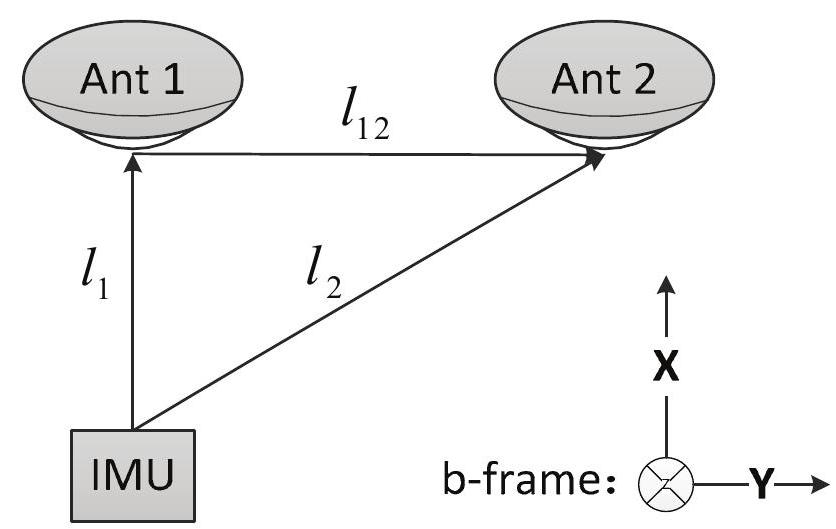
\includegraphics[max width=\textwidth]{2023_06_04_c79b87a911fb798e1754g-2}
\end{center}

Figura 1. Relația dintre locația fizică dintre unitatea de măsurare inerțială (IMU) și două antene de recepție ale sistemului global de navigație prin satelit (GNSS) din cadrul corpului.

Unde $l_{i}$ este vectorul brațului de nivel dintre IMU și $i$-a antena, în timp ce $l_{12}$ este vectorul brațului de nivel dintre cele două antene și poate fi exprimat astfel:

\begin{equation}
  l_{12}=l_{2}-l_{1}
\end{equation}


Ecuația de măsurare a erorii de poziție liniarizată este:

\begin{equation}
  \Delta \mathbf{Z}_{r}=r_{\mathrm{IMU}}-r_{\mathrm{GPS} 1}+C_{\mathrm{b}}^{\mathrm{n}} \boldsymbol{l}_{1}=\delta \boldsymbol{r}+\left(C_{\mathrm{b}}^{\mathrm{n}} \boldsymbol{l}_{1} \times\right) \psi-\boldsymbol{e}_{\widetilde{r}_{1}}
\end{equation}


unde $\Delta$ denotă diferența dintre măsurători și predicții. Ecuația de măsurare a erorii de viteză liniarizată este:

\begin{equation}
  \begin{aligned}
    \Delta \mathbf{Z}_{v} & =\left(\boldsymbol{v}_{\mathrm{IMU}}+\left(C_{\mathrm{b}}^{\mathrm{n}}\left(\boldsymbol{\omega}^{\mathrm{b}} \times\right)-\left(\omega_{\mathrm{in}} \times\right)\right) C_{\mathrm{b}}^{\mathrm{n}} \boldsymbol{l}_{1}-\boldsymbol{v}_{\mathrm{GPS} 1}\right)                                                                                                                                                                                                                                                                                                      \\
                          & =\delta \boldsymbol{v}-\left(\left(\boldsymbol{\omega}_{\mathrm{in}} \times\right) \boldsymbol{C}_{\mathrm{b}}^{\mathrm{n}}\left(\boldsymbol{l}_{1} \times\right)+C_{\mathrm{b}}^{\mathrm{n}}\left(\left(\boldsymbol{l}_{1} \times \omega^{\mathrm{b}}\right) \times\right)\right) \psi+C_{\mathrm{b}}^{\mathrm{n}}\left(\boldsymbol{l}_{1} \times\right) \boldsymbol{b}_{g}+C_{\mathrm{b}}^{\mathrm{n}}\left(\boldsymbol{l}_{1} \times\right) \operatorname{diag}\left(\boldsymbol{\omega}^{\mathrm{b}}\right) \boldsymbol{s}_{g}-\boldsymbol{e}_{\widetilde{v}_{1}}
  \end{aligned}
\end{equation}


unde $\bullet_{\mathrm{IMU}}$ și $\bullet_{\mathrm{GPS}}$ indică faptul că vectorii corespunzători sunt obținuți de algoritmul de mecanizare INS și, respectiv, algoritmul GPS-RTK. $(\bullet \times)$ denotă forma matriceală simetrică oblică a unui vector. $\boldsymbol{e}_{\widetilde{r}_{1}}$ și $\boldsymbol{e}_{\widetilde{v}_{1}}$ sunt vectorii de zgomot alb de măsurare corespunzători. $\omega_{\text {in }}$ este vectorul vitezei de rotație și este exprimat ca:

\begin{equation}
  \omega_{\text {in }}=\omega_{\text {ie }}+\omega_{\text {en }}
\end{equation}


Conform ecuației (7), o altă ecuație de măsurare a erorii de poziție legată de Rover 2 poate fi construită după cum urmează:

\begin{equation}
  \Delta \mathbf{Z}_{r}=\boldsymbol{r}_{\mathrm{IMU}}-\boldsymbol{r}_{\mathrm{GPS} 2}+C_{\mathrm{b}}^{\mathrm{n}} \boldsymbol{l}_{2}=\delta \boldsymbol{r}+\left(\boldsymbol{C}_{\mathrm{b}}^{\mathrm{n}} \boldsymbol{l}_{2} \times\right) \psi-\boldsymbol{e}_{\widetilde{r}_{2}}
\end{equation}


unde $e_{\widetilde{r}_{2}}$ este vectorul de zgomot alb de măsurare corespunzător.

$l_{12}$ a fost deja calibrat cu precizie în cadrul b și este considerat o constrângere care poate fi utilizată pentru fixarea rapidă a AR, chiar și pentru un receptor cu o singură frecvență cu costuri reduse. Să presupunem că vectorul liniei de bază cu două antene $p_{12}^{\mathrm{e}}$ în cadrul pământului (cadru e) poate fi estimat cu precizie prin procesarea GPS-RTK a receptorului de referință în mișcare pe care o folosește o metodă pentru determinați vectorul de poziție relativă între antene montate pe o singură platformă. Apoi, ecuația de măsurare a erorii de atitudine poate fi construită folosind diferența dintre ecuațiile (7) și (10):

\begin{equation}
  \begin{aligned}
    \Delta \mathbf{Z}_{\psi} & =\boldsymbol{r}_{\mathrm{IMU}}+C_{\mathrm{b}}^{\mathrm{n}} \boldsymbol{l}_{1}-\boldsymbol{r}_{\mathrm{GPS} 1}-\left(\boldsymbol{r}_{\mathrm{IMU}}+C_{\mathrm{b}}^{\mathrm{n}} \boldsymbol{l}_{2}-\boldsymbol{r}_{\mathrm{GPS} 2}\right) \\
                             & =C_{\mathrm{b}}^{\mathrm{n}} \boldsymbol{l}_{12}-C_{\mathrm{e}}^{\mathrm{n}} \boldsymbol{p}_{12}^{\mathrm{e}}                                                                                                                           \\
                             & =\left(C_{\mathrm{b}}^{\mathrm{n}} \boldsymbol{l}_{12} \times\right) \boldsymbol{\psi}-\boldsymbol{e}_{\widetilde{r}_{12}}
  \end{aligned}
\end{equation}

unde $\boldsymbol{e}_{\widetilde{r}_{12}}$ este secvența de zgomot alb de măsurare diferențială și $C_{\mathrm{e}}^{\mathrm{n}}$ este DCM de la e-frame la n-frame.

În consecință, modelul de eroare de măsurare de ordinul al nouălea al integrării GPS/INS cu două antene propuse este dat de:

\begin{equation}
  \Delta Z=H \delta x+e
\end{equation}


unde $\Delta Z$ este vectorul de măsurare, $H$ este matricea de măsurare calculată pe baza ecuațiilor (7), (8) și (11), $e$ este secvența de măsurare a zgomotului alb și, determinată de GPS /RTK, rezultă în variația erorii care reflectă incertitudinea de măsurare.

\begin{equation}
  \begin{aligned}
     & \Delta \mathbf{Z}=\left[\Delta Z_{r} \Delta Z_{v} \Delta Z_{\psi}\right]^{\mathrm{T}}                                                              \\
     & \boldsymbol{e}=\left[\boldsymbol{e}_{\widetilde{r}_{1}} \boldsymbol{e}_{\widetilde{v}_{1}} \boldsymbol{e}_{\widetilde{r}_{12}}\right]^{\mathrm{T}}
  \end{aligned}
\end{equation}


\begin{center}
  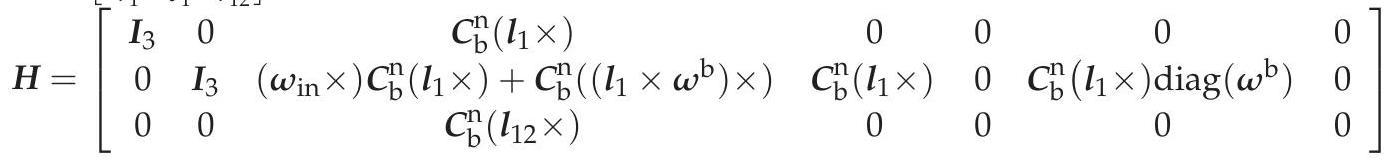
\includegraphics[max width=\textwidth]{2023_06_04_c79b87a911fb798e1754g-3}
\end{center}

unde $I_{3}$ este matricea unității de ordinul trei, 0 este matricea zero de ordinul trei.
\section{Adaptive Noise Covariance}
După cum s-a menționat în introducere, KF-urile au fost utilizate pe scară largă în fuziunea datelor, iar performanța lor se bazează pe acuratețea modelelor dinamice și de măsurare și pe acuratețea statistică a covarianței zgomotului $(Q$ și $R)$. Din fericire, $Q$ și $R$ pot fi încă ajustate pentru a reflecta incertitudinile reale ale estimării statului pe termen lung.

Matricea de covarianță a erorii de stare inițială reflectă acuratețea inițială a filtrarii stării, cu un efect redus asupra actualizării ulterioare a filtrului. Ponderea dintre $Q$ și $\boldsymbol{R}$ determină câștigul Kalman, care determină direct impactul pe care $Q$ și $R$ îl au asupra estimării stării. Prin urmare, focalizarea reconstrucției covarianței zgomotului este parțial deplasată către $\boldsymbol{Q}$ și $\boldsymbol{R}$.
\subsection*{Adaptive Process Noise Covariance}
Covarianța zgomotului de proces $Q$ ar trebui ajustată de algoritmul de filtru, deoarece nu poate fi controlată direct cu ușurință decât dacă factorul adaptiv $\alpha$ este utilizat pentru a regla covarianța stării prezise. $\boldsymbol{P}^{-}$poate fi exprimat ca:

\begin{equation}
  \boldsymbol{P}^{-}=\alpha\left(\boldsymbol{\Phi} \hat{\boldsymbol{P}} \boldsymbol{\Phi}^{\mathrm{T}}+\boldsymbol{Q} t\right)
\end{equation}

unde $\Phi$ denotă matricea de tranziție a stării calculată din sistemul dinamic INS, $t$ este timpul de discretizare și $\hat{\boldsymbol{P}}$ este covarianța stării actualizate la măsurarea anterioară. $\hat{\bullet}$ și $\bullet^{-}$indică parametrul actualizat de măsurare și, respectiv, parametrul prezis. $\alpha$ este o valoare scalară, actualizată pe baza ponderii dintre matricea de covarianță a vectorului rezidual prezis, notat cu $\hat{\mathcal{C}}_{\tilde{\xi}}$ și teoretic matricea de covarianță a vectorului rezidual prezis, notat cu $C_{\xi}$. $\hat{C}_{\xi}$ și $C_{\tilde{\xi}}$ sunt exprimate ca:

\begin{equation}
  \begin{aligned}
     & \boldsymbol{C}_{\tilde{\xi}}=\boldsymbol{H} \boldsymbol{P}^{-} \boldsymbol{H}^{\mathrm{T}}+\boldsymbol{R} \\
     & \hat{\boldsymbol{C}}_{\tilde{\xi}}=\boldsymbol{\xi}^{\mathrm{T}} \boldsymbol{\zeta}
  \end{aligned}
\end{equation}

unde $\xi$ este secvența inovației și exprimată ca:

\begin{equation}
  \xi=\mathbf{Z}-\mathbf{H} \delta \boldsymbol{x}^{-}
\end{equation}

cu succesiunea de stări prezise $\delta x^{-}$.

Pe baza principiului filtrului Kalman, $C_{\xi}$ reflectă eroarea de măsurare prezisă și teoretic este egal cu $\hat{C}_{\xi}$ într-un caz ideal (model dinamic și model de măsurare precis și statisticile lor de zgomot ). Să presupunem că măsurătorile sunt măsurate fără valori outlier și că funcțiile lor de densitate a probabilității de zgomot sunt precise.

Fie $\gamma=\operatorname{tr}\left(\hat{\boldsymbol{C}}_{\tilde{\xi}}\right) / \operatorname{tr}\left(\boldsymbol{C}_{ \xi}\right), \operatorname{tr}(\bullet)$ denotă urma unei matrice. Funcția adaptivă pentru determinarea factorilor adaptativi este exprimată ca:

\begin{equation}
  \alpha=\left\{\begin{array}{l}
    1.0, \gamma \leq \mathrm{c}_{0} \\
    \frac{1}{\mathrm{c}_{0}} \gamma, \mathrm{c}_{0} \leq \gamma
  \end{array}\right.
\end{equation}


unde $c_{0}$ este constanta empirică corespunzătoare, care este de obicei egală cu 1,5 -- 2,0 conform Referinței.

În condițiile unor măsurători precise sau statistici precise de zgomot, actualizarea timpului KF tinde să fie instabilă când $\alpha>1.0 . \mathbf{P}^{-}$este perturbat din cauza erorilor de model dinamic și ar trebui ajustat mai mare folosind $\alpha$ pentru a se asigura că $P^{-}$reflectează îndeaproape situația actuală.
\subsection*{Adaptive Measurement Noise Covariance}
Modificarea adaptivă a covarianței zgomotului este un compromis între rata de convergență și stabilitatea filtrului. Propagarea erorii de filtru reflectă într-o oarecare măsură acuratețea estimărilor stării. Într-o aplicație KF ideală, reglarea modelelor de zgomot pentru a genera erori și incertitudini de estimare consistente poate produce, de asemenea, estimări stabile ale stării care urmăresc adevăratele lor omologii. $\alpha$ face $P^{-}$mai mare și astfel determină creșterea valorii câștigului filtrului, ceea ce crește contribuția valorii outlier de măsurare. Valoarea anormală de măsurare $\delta \xi$ poate fi considerată incertitudinea necunoscută sau neidentificată conținută în inovație:

\begin{equation}
  \widetilde{\xi}=\xi+\delta \xi
\end{equation}

Conform ecuației (17), propagarea erorii de stare prezisă $\boldsymbol{P}^{-}$ poate fi mărită de $\beta$ ori fără $\delta \xi$ sau mărită incorect de $\alpha$ ori cu $\ delta \xi$ şi

\begin{equation}
  \begin{aligned}
    \beta & =\frac{\left.(\xi+\delta \xi)^{\mathrm{T}}(\xi) \delta \xi\right)}{\operatorname{tr}\left(\mathcal{C}_{\tilde{\xi}}\right)} / \frac{\xi^{\mathrm{T}} \boldsymbol{\xi}}{\operatorname{tr}\left(C_{\tilde{\xi}}\right)} \\
          & =1+\left(2 \delta \xi^{\mathrm{T}} \boldsymbol{\xi}+\delta \xi^{\mathrm{T}} \delta \xi\right) / \xi^{\mathrm{T}} \boldsymbol{\xi}
  \end{aligned}
\end{equation}


În procedura de actualizare a măsurătorilor, câștigul Kalman $K$ este calculat prin:

\begin{equation}
  \boldsymbol{K}=\boldsymbol{P}^{-} \boldsymbol{H}^{\mathrm{T}}\left(\boldsymbol{H} \boldsymbol{P}^{-} \boldsymbol{H}^{\mathrm{T}}+\boldsymbol{R}\right)^{-1}
\end{equation}


Actualizarea măsurătorilor estimării stării $\delta \hat{x}$ se formulează după cum urmează:

\begin{equation}
  \delta \hat{x}=\delta x^{-}+K \widetilde{\xi}=\delta x^{-}+K(\xi+\delta \xi)
\end{equation}


O mare parte a perturbațiilor din măsurare este transmisă înapoi la estimările stării deoarece valoarea câștigului corespunzătoare poate fi apropiată de 1,0, sub rezerva mărimii mari a erorii $\boldsymbol{P}^{-}$.

Dacă apar valori outlier ale măsurătorilor extreme, $\delta \xi$ tinde să fie extrem de mari. Apoi,

\begin{equation}
  \mid \frac{\delta \boldsymbol{\xi}^{\mathrm{T}} \delta \boldsymbol{\xi}}{\operatorname{tr}\left(\boldsymbol{H} \boldsymbol{P}^{-} \boldsymbol{H}^{\mathrm{T}}+\boldsymbol{R}\right)} \rightarrow \infty
\end{equation}

În comparație cu $R$ necorectat, $\xi$ conține erori de mare magnitudine. Prin urmare, $\alpha$ tinde să fie extrem de mare. Pentru o analiză mai intuitivă a dezavantajului erorilor mari de măsurare în $\widetilde{\xi}$, presupunem că $\alpha$ poate fi considerat că tinde spre infinit. Pe baza regulii lui L'Hôpital, câștigul Kalman corespunzător poate fi derivat ca:

\begin{equation}
  \begin{aligned}
    \lim _{\delta v \rightarrow \varepsilon} \boldsymbol{K} & =\lim _{\alpha \rightarrow \infty} \boldsymbol{K}                                                                                                                                                                                                      \\
                                                            & =\lim _{\alpha \rightarrow \infty} \alpha \boldsymbol{P}^{-} \boldsymbol{H}^{\mathrm{T}}\left(\boldsymbol{H} \alpha \boldsymbol{P}^{-} \boldsymbol{H}^{\mathrm{T}}+\boldsymbol{R}\right)^{-1}                                                          \\
                                                            & =\left[\partial\left(\alpha \boldsymbol{P}^{-} \boldsymbol{H}^{\mathrm{T}}\right) / \partial \alpha\right]\left[\partial\left(\boldsymbol{H} \alpha \boldsymbol{P}^{-} \boldsymbol{H}^{\mathrm{T}}+\boldsymbol{R}\right) / \partial \alpha\right]^{-1} \\
                                                            & =\boldsymbol{P}^{-} \boldsymbol{H}^{\mathrm{T}}\left(\boldsymbol{H} \boldsymbol{P}^{-} \boldsymbol{H}^{\mathrm{T}}\right)^{-1}
  \end{aligned}
\end{equation}


Conform ecuației (13), fiecare bloc al matricei $H P^{-} \boldsymbol{H}^{\mathrm{T}}$ constă din transformarea liniară a matricelor cu simetrie oblică, a căror determinare este egală cu 0 . Prin urmare, se pot produce blocări ale filtrului datorită inversării matricei singulare în porțiunea câștigului Kalman. Acest caz rareori există în general, deoarece determinarea lui $R$ nu este egală cu 0 și problemele numerice nu pot fi cauzate la procesarea inversării matricei în ecuația (23). Cu toate acestea, atunci când mărimea valorii outlier ale măsurării este mult mai mare decât mărimea lui $R$, contribuția lui $R$ la calculul câștigului poate fi degradată, chiar ignorată, iar feedback-ul pozitiv, divergența filtrului, chiar și problema numerică încă există. Micile erori în $P^{-}$sunt relativ inofensive; cu toate acestea, Ecuația (13) demonstrează că erorile mari ale matricei $P^{-}$ distorsionează matricea câștigului Kalman. $R$ este adesea reglat prin atribuirea de incertitudini de stare care sunt substanțial mai mari într-o măsură aproape echivalentă cu $\xi \xi^{\mathrm{T}}$ și covarianța modificată a zgomotului de măsurare care conține incertitudini necunoscute $\bar{R}$ poate fi exprimat ca:

\begin{equation}
  \overline{\boldsymbol{R}}=(\boldsymbol{s}+\boldsymbol{\rho})(\boldsymbol{s}+\boldsymbol{\rho})^{\mathrm{T}}
\end{equation}

unde secvența $\varsigma$ indică incertitudinea statistică inexactă și este empiric mai mică decât incertitudinile reale de măsurare. Secvența $\rho$ reprezintă incertitudinile de măsurare necunoscute, care se presupune că corespund aproximativ cu valorile outlier reale. Astfel, factorul de adaptare este:

\begin{equation}
  \alpha=\frac{\gamma}{\mathrm{c}_{0}}=\frac{1}{\mathrm{c}_{0}} \frac{\xi^{\mathrm{T}} \boldsymbol{\xi}+2 \delta \xi^{\mathrm{T}} \boldsymbol{\xi}+\delta \xi^{\mathrm{T}} \delta \xi}{\operatorname{tr}\left(\boldsymbol{H} \boldsymbol{P}^{-} \boldsymbol{H}^{\mathrm{T}}\right)+\boldsymbol{\varsigma}^{\mathrm{T}} \boldsymbol{\varsigma}+2 \boldsymbol{\varsigma}^{\mathrm{T}} \boldsymbol{\rho}+\boldsymbol{\rho}^{\mathrm{T}} \boldsymbol{\rho}}
\end{equation}


Dacă se stabilește ipoteza ecuației (22), se poate folosi regula lui L'Hôpital pentru a determina $\alpha$ și rezultă că:

\begin{equation}
  \alpha=\frac{\gamma}{\mathrm{c}_{0}}=\frac{1}{\mathrm{c}_{0}} \frac{\partial\left(\boldsymbol{\xi}^{\mathrm{T}} \boldsymbol{\xi}+2 \delta \xi^{\mathrm{T}} \boldsymbol{\xi}+\delta \boldsymbol{\xi}^{\mathrm{T}} \delta \boldsymbol{\xi}\right)}{\partial\left(\operatorname{tr}\left(\boldsymbol{H} \boldsymbol{P}^{-} \boldsymbol{H}^{\mathrm{T}}\right)+\boldsymbol{\varsigma}^{\mathrm{T}} \boldsymbol{\varsigma}+2 \boldsymbol{\varsigma}^{\mathrm{T}} \boldsymbol{\rho}+\boldsymbol{\rho}^{\mathrm{T}} \boldsymbol{\rho}\right)}=\frac{1}{\mathrm{c}_{0}} \frac{\|\boldsymbol{\xi}\|_{2}+\mid \delta \boldsymbol{\delta} \|_{2}}{\|\boldsymbol{\xi}\|_{2}+\|\boldsymbol{\rho}\|_{2}}
\end{equation}


unde $\|\bullet\|_{2}$ indică două norme ale unui vector.

Datorită introducerii $\rho$, contribuția valorii outlier de măsurare este aproape redusă cu

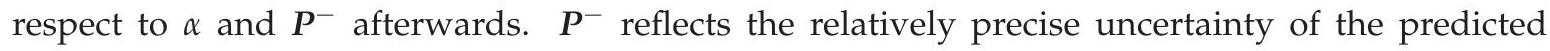
\includegraphics[max width=\textwidth, center]{2023_06_04_c79b87a911fb798e1754g-5}
estimările de stare și nu pot fi extrem de mari. Prin urmare, regula lui L'Hôpital nu poate fi utilizată în implementarea ecuației (23), probleme numerice privind inversarea lui $\left(\alpha \boldsymbol{H P}^{-} \boldsymbol{H}^{\mathrm{T }}+\overline{\boldsymbol{R}}\right)^{-1}$ sunt rezolvate, iar impactul feedback-ului pozitiv este atenuat datorită luării în considerare a incertitudinilor de măsurare necunoscute în determinarea câștigului Kalman. Cu toate acestea, $\rho$ este greu de separat; Cea mai populară metodă robustă din IAE este de a regla $\alpha$ în continuare folosind o funcție robustă adaptivă care este exprimată ca:

\begin{equation}
  \alpha=\left\{\begin{array}{cc}
    1.0,                                                                                                          & \gamma \leq \mathrm{c}_{0}                     \\
    \frac{\gamma}{\mathrm{c}_{0}} \times\left(\frac{\mathrm{c}_{1}-\mathrm{c}_{0}}{\mathrm{c}_{1}-\gamma}\right), & \mathrm{c}_{0} \leq \gamma \leq \mathrm{c}_{1} \\
    \frac{\mathrm{c}_{1}}{\gamma},                                                                                & \mathrm{c}_{1} \leq \gamma
  \end{array}\right.
\end{equation}


unde $c_{1}$ este constanta empirică corespunzătoare, care este de obicei egală cu 4,5-8,5.

Din păcate, există încă unele dezavantaje din următoarele motive:

\begin{itemize}
  \item Când reglați un filtru Kalman, incertitudinile necunoscute nu pot fi separate cu ușurință de zgomotul de măsurare. Deși stabilitatea filtrului este asigurată prin atribuirea unor incertitudini de stare substanțial mai mari, se introduce presupunerea subiectivă.

  \item Performanța ecuațiilor de eroare de măsurare în calibrarea INS este slăbită atunci când măsurarea este în starea de echilibru și nu poate oferi continuu rezultate de poziționare și viteză de înaltă precizie. Din cauza erorilor de model dinamic și a dezavantajelor mecanizării INS, INS nu poate oferi predicție precisă a stării. Datorită soluțiilor a priori cu precizie scăzută sau întreruperilor GPS, $\gamma$ poate fi, de asemenea, extrem de mare chiar și fără un valori aberanți de măsurare, deoarece ecuația (27) nu poate afla sursa abaterii mai mari ale inovației. Prin urmare, $\alpha$ poate fi mai mic de 1,0, iar impactul erorii $\boldsymbol{P}^{-}$matricei este crescut. Conform ecuațiilor (21) și (23), o eroare mică $\boldsymbol{P}^{-}$matricei produce estimări de stare care nu răspund, în timp ce $\boldsymbol{P}^{-}$de o magnitudine prea mare a erorii produce estimări instabile, oscilatorii de stare.

\end{itemize}

Contribuțiile $\boldsymbol{P}^{-}$și $\boldsymbol{R}$ determină impactul modelelor dinamice și, respectiv, de măsurare asupra estimării stării. Urmând ecuațiile (17) și (27), modificarea adaptivă a $\boldsymbol{P}^{-}$se bazează pe $\boldsymbol{R}$, ceea ce demonstrează că accent ar trebui pus pe detectarea valorii aberante ale măsurării și pe feedback. Prin urmare, Figura 2 ilustrează algoritmul propus utilizat pentru a determina $\rho$ în ecuația (24). În aplicația de navigație integrată GPS/INS cu două antene, $\boldsymbol{R}$ original este modificat pe baza procesării soluției de covarianță actualizate prin măsurarea filtrului de către GPS-RTK și reflectă acuratețea filtrului soluției GPS-RTK în detaliu $\left(\delta \widetilde{r}_{\mathrm{GPS}} \in \Re^{3 \times 1}, \delta \widetilde{v}_{\mathrm{GPS}} \in \Re^{3 \times 1}\right.$ și $\left.\delta \widetilde{\boldsymbol{p}}_{\mathrm{GPS}} \in \Re^{3 \times 1}\right) . \rho \in \Re^{3 \times 1}$ este proiectat pe baza valorii diluției de poziție a preciziei (PDOP), a numărului de sateliți valoroși (Nsat), a raportului AR și a prejudiciului de lungime $(d l)$ de $\widetilde {\boldsymbol{p}}_{12}$ care poate fi obținut prin procesarea GPS-RTK. Acești parametri pot reflecta în mod obiectiv calitatea soluțiilor RTK, ceea ce se îmbunătățește și pentru modificarea matricei de covarianță a zgomotului de măsurare și determinarea factorilor de adaptare. Pentru a regla matricea de covarianță a zgomotului de măsurare astfel încât să se alinieze îndeaproape cu mărimile reale ale erorii, $\bar{R}$ modificat este dat de:

\begin{equation}
  \begin{gathered}
    \overline{\boldsymbol{R}}=E\left[\boldsymbol{e} \boldsymbol{e}^{\mathrm{T}}\right] \\
    \boldsymbol{e}=\operatorname{diag}\left[\left(\delta \widetilde{\boldsymbol{r}}_{\mathrm{GPS}}+\boldsymbol{\rho}_{r}\right)\left(\delta \widetilde{\boldsymbol{v}}_{\mathrm{GPS}}+\boldsymbol{\rho}_{v}\right)\left(\delta \widetilde{\boldsymbol{p}}_{\mathrm{GPS}}+\rho_{\widetilde{\boldsymbol{p}}}\right)\right]^{\mathrm{T}}
  \end{gathered}
\end{equation}


unde $\boldsymbol{\rho}_{r}=\left[\rho_{r} \rho_{r} \rho_{r}\right]^{\mathrm{T}}, \boldsymbol{\rho}_ {v}=\left[\rho_{v} \rho_{v} \rho_{v}\right]^{\mathrm{T}}$ și $\boldsymbol{\rho}_{\widetilde{\boldsymbol{ p}}}=\left[\rho_{\widetilde{\boldsymbol{p}}} \rho_{\widetilde{\boldsymbol{p}}} \rho_{\widetilde{\boldsymbol{p}}}\right] ^{\mathrm{T}}$

$d l(<\Delta)$ mărginit este dat de:

\begin{equation}
  d l=\left\|\widetilde{\boldsymbol{p}}_{12}\right\|_{2}-\left\|\boldsymbol{l}_{12}\right\|_{2}
\end{equation}


Figura 2 prezintă algoritmul pentru modificarea adaptivă a matricei de covarianță a zgomotului de măsurare. Factorii $(\kappa, \mu, \gamma, \eta)$ prezentați în figură pot cuantifica fiabilitatea GPS-RTK în detaliu pentru a regla în mod corespunzător matricea de covarianță a zgomotului de măsurare.

\begin{center}
  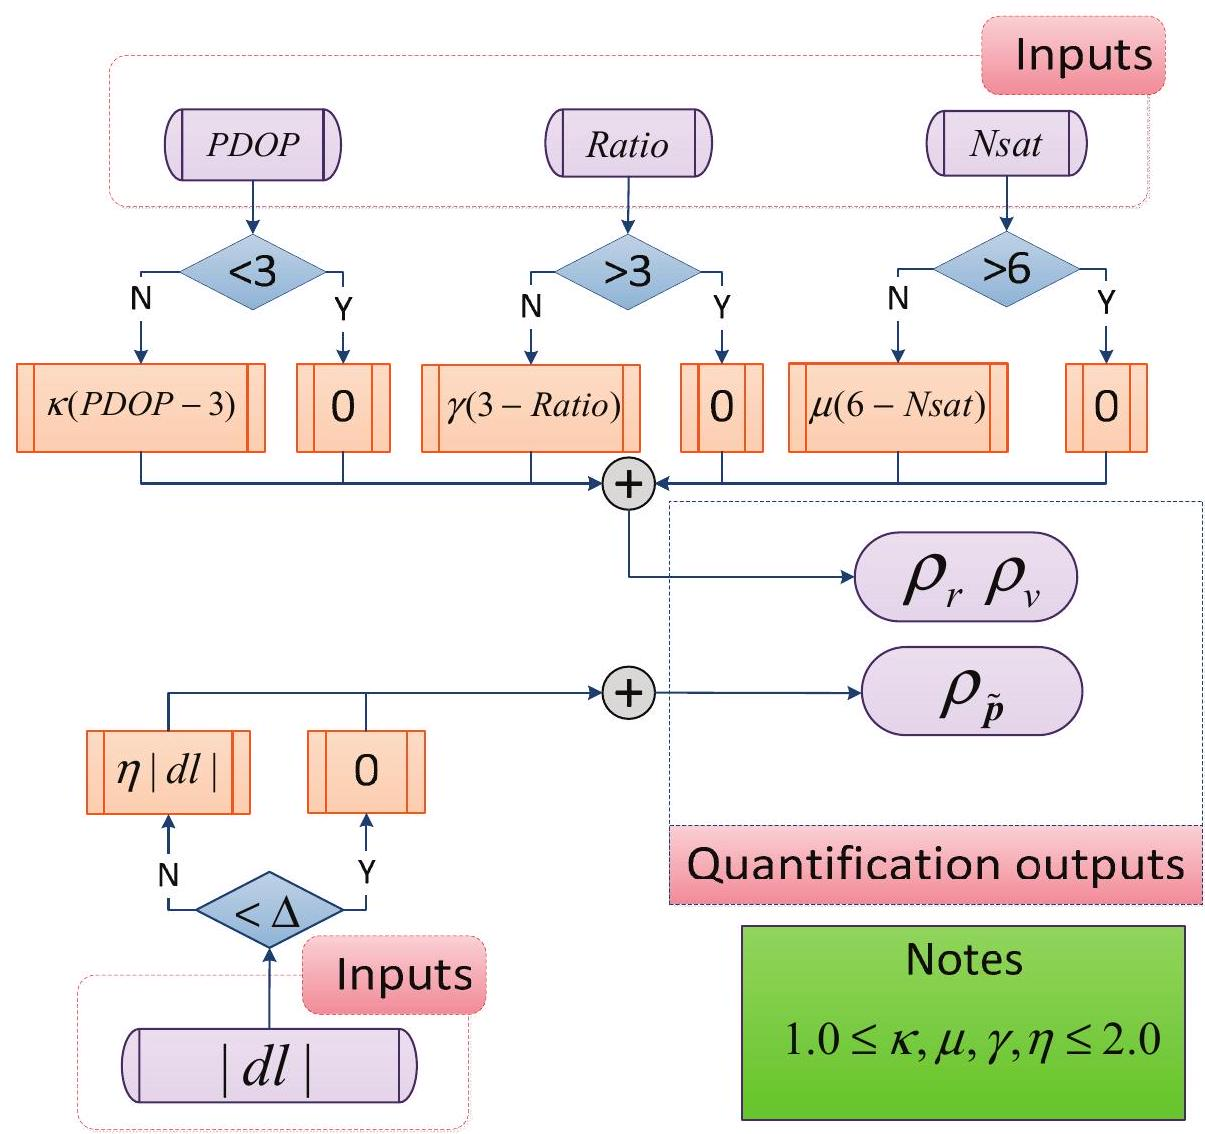
\includegraphics[max width=\textwidth]{2023_06_04_c79b87a911fb798e1754g-7}
\end{center}

Figura 2. Un algoritm de cuantificare a fiabilității Sistemului de poziționare globală (GPS)-RTK utilizat în ecuația (28) bazat pe PDOP, numărul de sateliți valoroși, raportul și părtinirea lungimii.

Conform figurii 2, algoritmul de reconfigurare a matricei de covarianță a zgomotului de măsurare adaptivă este formulat ca următoarea ecuație. Algoritmul este utilizat pentru a determina starea de conducere sau fiabilitatea măsurării pe baza rezultatelor cuantificării $\left(\rho_{r}, \rho_{v}\right.$ și $\left.\rho_{\tilde{p}} \right)$, care poate fi egal sau apropiat de 0 atunci când soluția GPS-RTK este fiabilă. În caz contrar, incertitudinile de stare mai mari de $1 \delta$ pot apărea în cazul în care măsurarea este mai puțin fiabilă. Factorii menționați în Figura 2, cum ar fi PDOP și raportul, sunt direct legați de performanța de poziționare; prin urmare, metoda propusă de modificare a matricei de covarianță a zgomotului de măsurare este mai fezabilă și mai flexibilă în comparație cu metoda robustă adaptivă din ecuația (27).

\begin{equation}
  \begin{aligned}
    \rho_{r}, \rho_{v} & =\kappa(P D O P-3)+\gamma(3-\text { Ratio })+\mu(6-\text { Nsat }) \\
    \rho_{\tilde{p}}   & =\eta|d l|
  \end{aligned}
\end{equation}

În rezumat, diagrama generală a algoritmului de integrare GPS/INS cu două antene este prezentată în Figura 3. Ieșirile IMU sunt procesate de algoritmul de mecanizare INS în parametrii de navigare, inclusiv vectorii de poziție, viteza, atitudine și vectorul de bază derivat $ C_{\mathrm{b}}^{\mathrm{n}} \boldsymbol{l}_{12}$ între cele două antene. Au fost adoptate două scheme de procesare GPS-RTK pentru a estima vectorii de poziție și viteză ai Rover-ului 1 și vectorul de linie de bază cu două antene $p_{12}^{\mathrm{n}}$. În această cercetare, implementarea implică un filtru bazat pe abordarea propusă.

\end{document}